\documentclass{article}
\usepackage{amsmath}
%\usepackage{psfig}

\usepackage{amsmath}
\usepackage{graphicx}
\usepackage{float}
\usepackage{amssymb} 
\usepackage{amsthm}
\usepackage{pgf}
\usepackage{tikz}
\usetikzlibrary{automata,shapes.multipart} %
\usetikzlibrary{arrows,petri}
\usepackage[latin1]{inputenc}
%\usepackage[noend]{algorithmic}
\usepackage{algorithm}
%\usepackage{algo}
\usepackage{epsfig}
\usepackage{subfigure}
\usepackage{multirow}
\usepackage{url}
\usepackage{syntax}


\newcommand{\cosmos}{\mbox{\textup{C}\scalebox{0.75}{{\textsc{OSMOS}}}}}
\newcommand{\cosyverif}{\mbox{\textup{C}\scalebox{0.75}{{\textsc{OSY}}}\textup{V}\scalebox{0.75}{{\textsc{ERIF}}}}}

\title{\cosmos{} User Manual}
\author{Beno\^it Barbot}

\begin{document}
\maketitle


This is the user manual for the tool \cosmos{} version 1.4

\section{Tool Usage}

\subsection{Basic Usage}
The primary usage of the tool \cosmos{} is as follow:
\begin{verbatim}
Cosmos model property
\end{verbatim}
where the model is specified in the GRML file format or in the
\verb|.grml| file format and the property is expressed either in GRML
or in the \verb|.lha| file format.

\subsubsection{Model}
Models taken by \cosmos{} as input are variant of Petri net.  The main
model supported by \cosmos are Stochastic Petri net with inhibitor
arcs and general distribution. The file format of \cosyverif{} (GRML) 
allows to specified different variant of Petri Net which are also 
recognize by \cosmos{}:
\begin{itemize}
\item Plain Petri net can be read in this case exponential distribution of 
  rate $1$ is assign to each transition.
\item Stochastic Petri net with inhibitor arc and general distribution.
\item Symmetric Net, like for plain Petri net in this case exponential
  distribution of rate $1$ are assume.
\item Stochastic Symmetric Net. 
\end{itemize}
The specification of file format are reported in Section~\ref{sec:fileformat}.

\subsubsection{Property}
Property are specified in the Hybrid Linear Automaton Logic(HASL)
which as the name suggest relies on Linear Hybrid Automaton(LHA) to
select path and on several HASL expression to specify various
performance values.

\subsection{Statistical Options}
Several options can be used to control the behaviors of the statistical engine.
The default behaviors is to simulate trajectories until either
\begin{itemize}
\item The maximum number of trajectories is reach.
\item The specified width for confidence intervals is reach.
\end{itemize}

\subsubsection{\texttt{--width arg}  option}
This option specified \texttt{arg} as the objective width for
confidence intervals. If it is set to $0$ trajectories are
simulated until the maximum number of trajectories is reached.
The default value is $0.001$.

\subsubsection{\texttt{--max-run arg}  option}
This option specified \texttt{arg} as the maximal number of run.
The default value is $2,000,000$.

\subsubsection{\texttt{--level arg}  option}
This option set the confidence level to \texttt{arg}.
The default value is $0.99$.

\subsubsection{\texttt{--batch arg}  option}
This option set the number of simulation to perform between each
statistical test.  The default value is $1000$. When this value is 
set to $0$ the tool will perform a test at constant time period.

\subsubsection{\texttt{--njob arg}  option}
This option set the number of parallel computation to \texttt{arg}.
The default value is $1$.

\subsubsection{\texttt{--relative}  option}
This option set allow cosmos to used relative confidence interval
instead of absolute one.

\subsubsection{\texttt{--chernoff arg}  option}
This option use chernoff-hoeffding bound to compute statistical parameter.
\texttt{arg} contain one of \texttt{width,level,nbrun}. The parameter 
specified by \texttt{arg} is computed using Chernoff-Hoeffding bound.

\subsection{Input Options}

\subsubsection{\texttt{--const X1=c1,X2=c2,\dots,Xn=cn}  option}
This option overrides values of constants of models. The constants is
define if it was done define in the model before.

\subsubsection{\texttt{-g, --grml-input}  option}
This option force the tool to use the GRML parser for the model and
the LHA. This is mostly deprecated as the correct parser is inferred
from the extension.

\subsubsection{\texttt{--HASL-expression arg}  option}
This allow to specify additional HASL{} expressions to the automaton.
The syntax of \texttt{arg} is the one of HASL{} expression in the
\texttt{.lha} file format and should ends with ``\texttt{;}''.

\subsubsection{\texttt{--loop arg [--transient arg2]}  option}
This produce a set of HASL formulas evaluating the mean number of 
token in each place and the mean throughput of each transition until time
\texttt{arg}. The optional additional argument allows to specify a transient
time where the mean number of token and throughput are not recorded.
See option \texttt{--trace-place} to specify which places and transitions 
to monitor.

\subsubsection{\texttt{--sampling t1 t2} option}
This produce an automaton that sample each \texttt{t2} time unit the
mean number of token in each place for this period, until time
\texttt{t1} is reached.  See option \texttt{--output-graph} to format
the output in a more manageable way.

\subsubsection{\texttt{--count-transition} option}
This Produce a set of HASL formulas counting the number of firing of each
transition.

\subsubsection{\texttt{--formula arg} option}
Send the expression \texttt{arg} to the \emph{AutomataGen} tool to produce
the LHA used for the simulation. The tool AutomataGen is a work in progress.

\subsection{Output formatting Options}
The default behavior of \cosmos{} for displaying result is as follows:
During the simulation a synthetic overview is displayed:
\begin{scriptsize}
\begin{verbatim}
Total paths: 28570000  Accepted paths: 22442000  Wall-clock time: 21s  Remaining(approx): 32s  Trajectory per second: 1.4e+06
r:        |< 2.639128431e-08 --[ 0.4999066088    < 0.5000635601    > 0.5002205154    ]-- 0.9999999687    >| width=0.000313902
pi:       |< 0               --[ 3.141245613     < 3.142037101     > 3.142828210     ]-- 4               >| width=0.001582596
pi2:      |< 0               --[ 0.7853114033    < 0.7855092754    > 0.7857070525    ]-- 1               >| width=0.000395649
% of Err: [||||||||||||||||||||||||||||||||||||||||                                                       ] 39%	
% of run: [||||||||||||||||||||||||||||                                                                   ] 28%	
\end{verbatim}
\end{scriptsize}
The first line provide information on the speed of simulation. The
remaining time is computed assuming that the size of confidence
interval decrease in $1/\sqrt{N}$ with $N$ the number of trajectories.
The second to fourth line present three HASL expressions. The first
number is minimal value observed for this expression, then the lower
bound of the confidence interval is displayed, then the estimated
value, then the upper bound and then the maximal observed value. The
width of the confidence interval is displayed at the end.  The last
two lines show progress bar indicating the progress of the
simulation. The first one indicate the progress to reach specified
confidence interval width limit. This progress is corrected assuming
that the width progress in $1/\sqrt{N}$ thus this bar progress at
constant speed. The last bar is the number of simulated trajectory 
compare to the maximal number of trajectories.

When the simulation finished results are return in key-value format
easier to parse for tools:
\begin{scriptsize}
\begin{verbatim}
Model path:	pi.gspn
LHA path:	pi.lha
r:
Estimated value:	0.500031454383448
Confidence interval:	[0.499932270760877 , 0.50013063800602]
Minimal and maximal value:	[1.93365088646926e-08 , 0.999999971987635]
Width:	0.000198367245143327
pi:
Estimated value:	3.14176752504576
Confidence interval:	[3.14126745104347 , 3.1422674472686]
Minimal and maximal value:	[0 , 4]
Width:	0.000999996225129696
pi2:
Estimated value:	0.78544188126144
Confidence interval:	[0.785316862760866 , 0.785566861817149]
Minimal and maximal value:	[0 , 1]
Width:	0.000249999056282424
Method:	Confidence interval computed sequentially using Chows-Robbin algorithm or SPRT.
Confidence level:	0.99
Total paths:	71569000
Accepted paths:	56213290
Batch size:	1000
Time for simulation:	55.245259s
Total CPU time:	60.068667
Total Memory used:	44.87 MB
Number of jobs:	1
Results are saved in 'Result_pi.res'
Results are saved in 'Result.res'
\end{verbatim}
\end{scriptsize}
All the simulations parameters are recalled. The additional
information are the \texttt{Time for simulation} which is the wall
clock time uses by the simulation.  It decrease when the number of
parallel processes increases on multi-processor machine.  The
\texttt{Total CPU time} is the cpu time consume by the whole
computation it slightly increases when the number of parallel process
increases. The \texttt{Total Memory used} line report the memory used
by the whole computation. In most cases the maximum memory consumption
is reached during the compilation of the simulator and highly depends of
the compiler used. This output is also stored in a file called \texttt{Result.res}.

Several option allow to output other data from the simulation:

\subsubsection{\texttt{-v, --verbose arg} option}
Set the verbose level of the tool. The default is $2$, with $0$ the tool
does not write anything on the standard output. The maximum is $6$ which 
generate debug information at each step of the simulation.

\subsubsection{\texttt{-i,--interactive} option}
This option allows to debug a model by stopping the simulation after
each step.  This is option should not be used together with
\texttt{--njob n} with $n>1$.  When the simulation is stopped the user
is asked either to type \texttt{step} to fire the following transition
or \texttt{fire tr} where \texttt{tr} is the name of an enabled
transition. This mode is not fully compatible with stochastic
symmetric net as the command \texttt{fire} does not allows to specify
a binding.

\subsubsection{\texttt{--output-graph arg} option}
Allows to output results of HASL formula in a blank separated file
format. The argument \texttt{arg} specify the name of the file.  This
is well suited for HASL expressions specifying a graph like
\texttt{PDF, CDF} or the expression generated by the
\texttt{--sampling} option.  Figure~\ref{fig:sampling} show a graph
generated by the \texttt{--sampling 2 0.001} option on the shared
memory example. The \texttt{--output-graph} option generate a file
starting as file:
\begin{scriptsize}
\begin{verbatim}
abscissa MeanToken_Access1_low MeanToken_Access1_mean MeanToken_Access1_up           ... 
0.005 7.6218e-05 0.000144057 0.000211896 0.00920415 0.00986402 0.0105239 0.000103712 ...
0.015 0.000803674 0.00103768 0.00127168 0.0279092 0.0292027 0.0304962 0.000759281    ...
...
\end{verbatim}
\end{scriptsize}
which can easily be plotted as the figure using \texttt{gnuplot}.
This can be used for user defined HASL formula by using name ending by
\verb|$GRAPH$x1$x2$| for HASL expressions where $(x1+x2)/2$ is the
abcsissa of the point computed by the expression.

\begin{figure}[h]
  \centering
  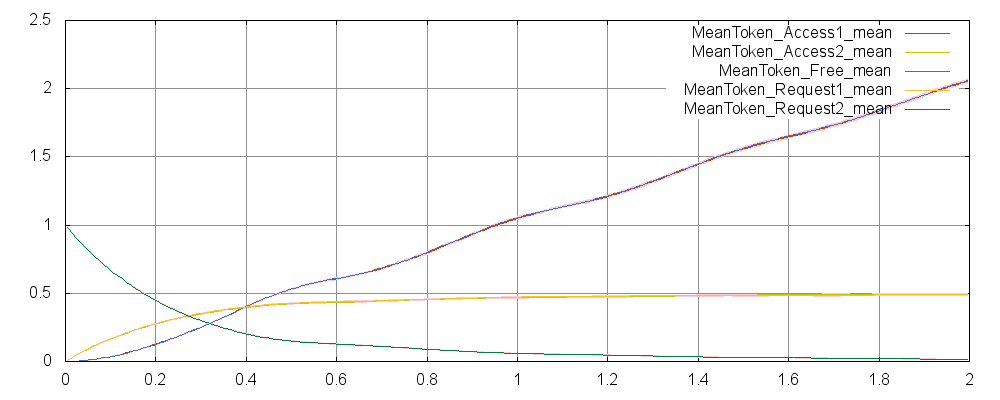
\includegraphics[width=1.01\textwidth]{figures/sampling.png}
  \caption{Sampling the trajectories of the shared memory example}
  \label{fig:sampling}
\end{figure}

\subsubsection{\texttt{-d, --output-data arg} option}
This option generate a file containing showing the evolution of 
confidence intervals along the time, this allow to observe the
speed of convergence. Figure~\ref{fig:convergence} shows a graph
plotted from these data. 

\begin{figure}[h]
  \centering
  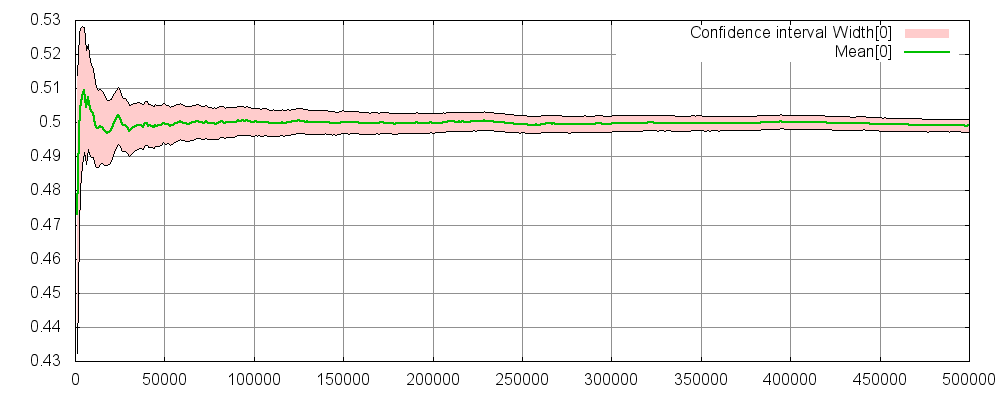
\includegraphics[width=1.01\textwidth]{figures/convergence.png}
  \caption{Convergence of the estimation for the shared memory example}
  \label{fig:convergence}
\end{figure}

\subsubsection{\texttt{--output-raw arg} option}
This option allows to output the end value of HASL expression at
the end of each trajectories. This option was introduced for debug 
purposes and should not be used in normal use. This option is not compatible
with \texttt{--njob n} when $n>1$

\subsubsection{\texttt{--output-trace arg arg2} option}
This option store traces of trajectories of simulation in file
\texttt{arg}.  Each line contains the global state of the simulator
(Petri net + LHA) after a transition.  Each trajectories are separated
by a line containing \texttt{New Path}.  Figure~\ref{fig:trace}
contains a trace of one trajectory of the shared memory example.  The
second argument \texttt{arg2} specify a minimum sampling time. If
\texttt{arg2} $>0$, no two lines in the output file are separated by
less than \texttt{arg2} time unit. This is useful when the trace
became to big to reduce the size of the generated file.

\begin{figure}[h]
  \centering
  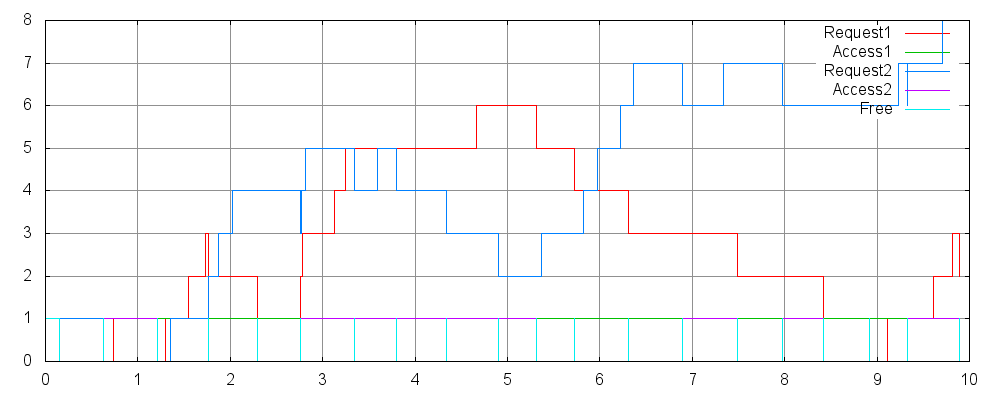
\includegraphics[width=1.01\textwidth]{figures/trace.png}
  \caption{Trace of one simulation for the shared memory example}
  \label{fig:trace}
\end{figure}

\subsubsection{\texttt{--trace-pt arg} option}
Specify which place and transition should be traced in the various
output file.  \texttt{arg} is a list of place and transition
name. There are two keyword \texttt{ALL} which is the default and
\texttt{COLOR}, the first allow to trace all places and transitions,
the second allow to trace all color token and all binding of
transition for stochastic symmetric net.

\subsubsection{\texttt{--gnuplot-driver} option}
This option makes \cosmos{} call \texttt{gnuplot} interactively and
display the graph of all output specify by a \texttt{--output-*}
option.  All the graph of this manual have been created using this
option.

\subsubsection{\texttt{--alligator-mode} option}
This option remove the output of the progress of the simulation 
and output progress as line containing key-value. This mode
is useful for interfacing cosmos with other tool in particular 
with \texttt{alligator} the server part of \cosyverif. This 
mode also makes the \texttt{--gnuplot-driver} option to write
the graph is files instead than on the screen.

\subsubsection{\texttt{--update-time arg} option}
This option set the time between two update of the progress of the simulation
to be no less than \texttt{arg}.

\subsection{Miscellaneous Options}
\subsubsection{\texttt{--version} option}
Display the current version of \cosmos{}.

\subsubsection{\texttt{-h, --help} option}
Display a help message containing the list of option and quit.

\subsubsection{\texttt{--seed arg} option}
Set the seed of the simulator to \texttt{arg}. 

\subsubsection{\texttt{--local-test} option}
This option change the way enabled transitions are computed.  This can
improve performance for net containing transitions with a lot of input
arcs.


\subsubsection{\texttt{--unfold arg} option}
This option output the model as a place transition net in the GrML
file format this allows to unfold Symmetric net but also to convert
\texttt{.gspn} file to GrML. This option is a work in progress some
expression on arcs may not be well exported.


\subsubsection{\texttt{-s, --state-space} option}
Do not run the simulator instead generate the state space and 
the transition probability matrix. The output format is the one
used by \texttt{Prism} to import models. 

\subsubsection{\texttt{--prism} option}
Export the state space then run \texttt{Prism} on it.
At the end of the computation the vector of probability to reach
accepting state is read and exported.

\subsubsection{\texttt{--gppcmd arg} option}
Set the C++ compiler to be \texttt{arg}.

\subsubsection{\texttt{--gppflags arg} option}
Appends \texttt{arg} to the command line calling the C++ compiler.

\subsection{Debugging Options}
The following options are implemented only for debugging purposes and
should not be used in general.

\subsubsection{\texttt{--tmp-status arg} option}
Change the way \cosmos{} handle temporary files. The argument \texttt{arg}
can takes four values: 
\begin{itemize}
\item $0$ is the default. A temporary directory is asked to the system
  all temporary files are generated in it. The directory is destroyed
  at the end of the computation.
\item $2$. The directory name \texttt{tmp} in the current
  \texttt{PATH} is used, it is not destroyed at the end. This option
  is useful to examine generated code.
\item $1$. \cosmos{} assume that the directory \texttt{tmp} exists
  and contains a fully build version of the model and property. The
  simulator is launched without being rebuild. At the end of computation
  the directory is destroyed.
\item $3$. Same as $1$ but do not destroyed the \texttt{tmp} directory
  at the end.
\end{itemize}
These option allows to build only once a model and reuse it for
several simulations. Only statistical parameters can be change between simulation
as the model is not rebuild. Use with caution!

\subsubsection{\texttt{--tmp-path arg} option}
Specify where to put the temporary directory. This option is useless
if the \texttt{--tmp-status arg} with \texttt{arg}$>0$ is not specify.

\subsubsection{\texttt{--bin-path arg} option}
Override the path to the installation of \cosmos{}. This path is used
by cosmos to find headers and libraries requires to build the model.

\subsubsection{\texttt{--debug-string} option}
Add debuging information to the generated code. This option is activated
and required by a verbose mode greater than $4$.

 

\section{File Format}
\label{sec:fileformat}

\subsection{GrML file format}
GrML for Graph Markup Language is the graph base language to define
models in the \cosyverif platform. This language is based on XML.


\subsection{Generalized Stochastic Petri Net (.gspn)}
This file format is used to describe GSPN.
First we describe an example:\\
\begin{figure}[h]
  \centering
  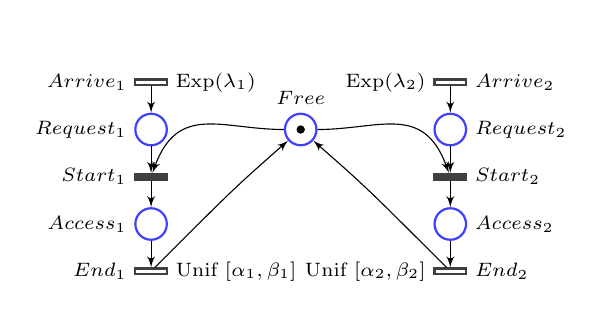
\begin{tikzpicture}[node distance=0.6cm,>=stealth',auto]
{\scriptsize
  \tikzstyle{place}=[circle,thick,draw=blue!75,minimum size=4mm]
  \tikzstyle{transition}=[rectangle,thick,draw=black!75,
  minimum width=4mm,inner sep=0pt,minimum height=.7mm]

    \node [] (i1)       {};
    \node [transition,label=left:$Arrive_1$,label=right:Exp($\lambda_1$)] (tr1) [below of =i1]{};
    \node [place,label=left:$Request_1$] (r1) [below of=tr1]  {};
    \node [transition,,label=left:$Start_1$,fill=black!75] (ta1) [below of =r1]{}; %label=right:$(\mbox{pri}_1\colon w_1)$
    \node [place,label=left:$Access_1$] (a1)  [below of=ta1] {};
    \node [transition,label=left:$End_1$,label=right:{\hspace{-0mm}{\scriptsize Unif $[\alpha_1,\beta_1]$}}] (ti1) [below of =a1]{};
    \node [place,tokens=1,label=above:$Free$] (f) [right of=r1,xshift=13mm]    {};
    \node [place,label=right:$Request_2$] (r2) [right of=f,xshift=13mm]    {};
   \node [transition,label=right:$Arrive_2$,label=left:Exp($\lambda_2$)] (tr2) [above of =r2]{};
    \node [] (i2) [above of=tr2]    {};
    \node [transition,label=right:$Start_2$,fill=black!75] (ta2) [below of =r2]{}; %label=left:$(\mbox{pri}_2\colon w_2)$,
    \node [place,label=right:$Access_2$] (a2) [below of=ta2]    {};
    \node [transition,label=right:$End_2$,label=left:{\hspace{-2mm}{\scriptsize Unif $[\alpha_2,\beta_2]$}}] (ti2) [below of =a2]{};
%\draw [-latex'] (i1) to (tr1);
\draw [-latex'] (tr1) to (r1);
\draw [-latex'] (r1) to (ta1);
\draw [-latex'] (ta1) to (a1);
\draw [-latex'] (a1) to (ti1);
%\draw [-latex'] (i2) to (tr2);
\draw [-latex'] (tr2) to (r2);
\draw [-latex'] (r2) to (ta2);
\draw [-latex'] (ta2) to (a2);
\draw [-latex'] (a2) to (ti2);
\draw [-latex'] (f) .. controls +(0:10mm) and +(110:10mm) .. (ta2);
\draw [-latex'] (f) .. controls +(180:10mm) and +(70:10mm) .. (ta1);
\draw [-latex'] (ti1) .. controls +(45:15mm)  .. (f); %and +(260:20mm)
\draw [-latex'] (ti2) .. controls +(135:15mm) .. (f); %and +(280:20mm) 
}
\end{tikzpicture} 
  \caption{Infinite-state GSPN  model of a shared memory system.}
  \label{fig:sharedmem}
  % \vspace*{-.3cm}
\end{figure}
This GSPN is described by the following text:

\begin{scriptsize}
\begin{verbatim}
const double lambda1 = 1;
const double lambda2 = 2;
const double alpha1 = 1;
const double alpha2 = 1;
const double beta1 = 5;
const double beta2 = 5;

NbPlaces = 5;
NbTransitions = 6;

PlacesList = { 
   Request_1, Request_2,
   Access_1, Access_2,
   Free
} ;

TransitionsList = { 
   Arrive_1,Arrive_2,
   Start_1 ,Start_2,
   End_1   ,End_2
} ;

Marking={
   (Request_1 , 0); (Request_2 , 0) ; 
   (Access_1 , 0) ; (Access_2 , 0) ;
   (Free, 1);
};

Transitions={
   (Arrive_1,EXPONENTIAL(lambda1),1,1, SINGLE); 
   (Arrive_2,EXPONENTIAL(lambda2),1,1, SINGLE);
   (Start_1,DETERMINISTIC(0),1,1); 
   (Start_2,DETERMINISTIC(0),1,1);
   (End_1,UNIFORM(alpha1,beta1),1,1); 
   (End_2,UNIFORM(alpha2,beta2),1,1);
};

InArcs={
   (Request_1,Start_1,1); (Free,Start_1,1);
   (Request_2,Start_2,1); (Free,Start_2,1);
   (Access_1,End_1,1);
   (Access_2,End_2,1);
};

OutArcs={
   (Arrive_1,Request_1,1); 
   (Arrive_2,Request_2,1);
   (End_1,Free,1);
   (End_2,Free,1);
};
\end{verbatim}
\end{scriptsize}

{\bf Description:}
The first bloc is a list of constants definition, constants can be
either \verb|double| or \verb|int|.\\
Then we specify the number of place and transitions with:
\verb|NbPlaces = 5; NbTransitions = 6;|\\
The list of place name and transition name is given in the
\verb|PlacesList| and \verb|TransitionsList| statement.\\
The initial marking of the net is given as a set of pairs
in the \verb|Marking| statement.\\
The transition distribution is given as a set of tuples like
this one:\\ \verb|(Arrive_1,EXPONENTIAL(lambda1),1,1, SINGLE)|
each tuple contain first the name of the transition then
the probability distribution with some parameters, then two positive
reals define the priority and weight of the event generated.
For exponential distribution we can specify the policy of service
which can be \verb|SINGLE,INFINITE,MULTIPLE(n)|.\\
Finally come the description of arcs of the net with the 
\verb|InArcs|,\verb|OutArcs| and \verb|InhibitorsArcs| statements.



\subsubsection{Grammar}
the complete grammar is:

\begin{scriptsize}
\begin{grammar}
<accept> ::= <GSPN> 'end of file'

<GSPN> ::= <declarations> <definitions>
 
<declarations> ::= <Constants> <Sizes> <Lists>
            | <Sizes> <Lists>

<Constants> ::= <Constant>
         | <Constant> <Constants>

<Constant> ::= 'const' 'int' <str> '=' IntStringFormula ';'
        | 'const' 'double' <str> '=' RealStringFormula ';'

<IntStringFormula> ::= <ival> | <str>
                \alt '(' <IntStringFormula> ')'
                \alt <IntStringFormula> '+' <IntStringFormula>
                \alt <IntStringFormula> '-' <IntStringFormula>
                \alt <IntStringFormula> '*' <IntStringFormula>
                \alt <IntStringFormula> '\^' <IntStringFormula>
                \alt FLOOR '(' <IntStringFormula> ')'
                \alt FLOOR '(' <IntStringFormula> '/' <IntStringFormula> ')'
                \alt MIN '(' <IntStringFormula> ',' <IntStringFormula> ')'
                \alt MAX '(' <IntStringFormula> ',' <IntStringFormula> ')'

<RealStringFormula> ::= <rval> | <ival> | <str>
                 \alt '(' <RealStringFormula> ')'
                 \alt <RealStringFormula> '/' <RealStringFormula>
                 \alt <RealStringFormula> '+' <RealStringFormula>
                 \alt <RealStringFormula> '-' <RealStringFormula>
                 \alt <RealStringFormula> '*' <RealStringFormula>
                 \alt <RealStringFormula> '\^' <RealStringFormula>
                 \alt FLOOR '(' <RealStringFormula> ')'
                 \alt MIN '(' <RealStringFormula> ',' <RealStringFormula> ')'
                 \alt MAX '(' <RealStringFormula> ',' <RealStringFormula> ')'

<Sizes> ::= <NbPlaces> <NbTransitions>
     | <NbTransitions> <NbPlaces>

<NbPlaces> ::= 'NbPlaces' '=' <ival> ';'
        | 'NbPlaces' '=' <str> ';'

<NbTransitions> ::= 'NbTransitions' '=' <ival> ';'
             | 'NbTransitions' '=' <str> ';'

<Lists> ::= <PlacesList> <TransitionsList>
     | <TransitionsList> <PlacesList>

<PlacesList> ::= 'PlacesList' '=' '{' <PLabels> '}' ';'

<PLabels> ::= <str>
       | <PLabels> ',' <str>

<TransitionsList> ::= 'TransitionList' '=' '{' <TLabels> '}' ';'

<TLabels> ::= <str>
       | <TLabels> ',' <str>

<definitions> ::= <PlacesDef> <TransitionsDef> <InArcs> <OutArcs>
           \alt <PlacesDef> <TransitionsDef> <InArcs> <OutArcs> <Inhibitors>

<PlacesDef> ::= 'Marking' '=' '{' <PLACES> '}' ';'

<PLACES> ::= <PLACE>
      | <PLACES> <PLACE>

<PLACE> ::= '(' <str> ',' <IntStringFormula> ')' ';'

<TransitionsDef> ::= 'Transition' '=' '{' <TRANSITIONS> '}' ';'

<Transitions> ::= <Transition>
           | <Transitions> <Transition>

<Transition> ::= '(' <str> ',' <dist> ',' <Priority> ',' <Weight> ')' ';'
          \alt '(' <str> ',' 'EXPONENTIAL' '(' <RealStringFormula> ')' ',' <Priority> ',' 
            <Weight> ',' <Service> ')' ';'
          \alt '(' <str> ',' 'IMDT' ',' <Priority> ',' <Weight> ')' ';'

<dist> ::= <str> '(' <params> ')'

<params> ::= <RealStringFormula>
      | <params> ',' <RealStringFormula>

<Weight> ::= <RealStringFormula>

<Priority> ::= <RealStringFormula>

<Service> ::= 'SINGLE'
       | 'INFINITE'
       | 'MULTIPLE' '(' <ival> ')'
       | 'MULTIPLE' '(' <str> ')'

<InArcs> ::= 'InArcs' '=' '{' <incells> '}' ';'

<incells> ::= <incell>
       | <incells> <incell>

<incell> ::= '(' <str> ',' <str> ',' <IntStringFormula> ')' ';'
      | '(' <str> ',' <str> ')' ';'

<OutArcs> ::= 'OutArcs' '=' '{' <outcells> '}' ';'

<outcells> ::= <outcell>
        | <outcells> <outcell>

<outcell> ::= '(' <str> ',' <str> ',' <IntStringFormula> ')' ';'
       | '(' <str> ',' <str> ')' ';'

<Inhibitors> ::= 'inhibitor' '=' '{' <inhibcells> '}' ';'

<inhibcells> ::= <inhibcell>
          | <inhibcells> <inhibcell>

<inhibcell> ::= '(' <str> ',' <str> ',' <IntStringFormula> ')' ';'
         | '(' <str> ',' <str> ')' ';'
\end{grammar}
\end{scriptsize}

\subsection{Linar Hybrid Automaton(.lha)}


\subsubsection{General Expression}

\begin{scriptsize}
\begin{grammar}
  <MarkingDepExpr> ::= <ConstIdentifier> | <DiscreteVarIdentifier> | <PlaceIdentifier>
  \alt  <MarkingDepExpr> `+'  <MarkingDepExpr> | <MarkingDepExpr> `-'  <MarkingDepExpr>
  \alt  <MarkingDepExpr> `*'  <MarkingDepExpr>
  \alt `Card' <MarkingDepExpr>
  \alt <MarkingDepExpr> `[' <ColorList> `]'
  \alt <DomainMarking>

 <Expr> ::= <ConstIdentifier> | <DiscreteVarIdentifier>  | <VarIdentifier> | <PlaceIdentifier>
  \alt  <Expr> `+'  <Expr> | <Expr> `-'  <Expr>
  \alt  <Expr> `*'  <Expr>
  \alt `Card' <Expr>
  \alt <Expr> `[' <ColorList> `]'
  \alt <DomainMarking>

  <ColorList> ::= <ColorExpr> `,' <ColorList>
  \alt <ColorExpr>

  <ColorExpr> ::= <ColorIdentifier> | <ColorVarIdentifier>
  \alt <ColorExpr> `++' | <ColorExpr> `--'

  <LinearExpr> ::= <LinearExpr> `+'  <LinearExpr> | <LinearExpr> `-'  <LinearExpr>
  \alt <MarkingDepExpr> `*' <VarExpr>

  <VarExpr> ::= <VarIdentifier> | <VarIdentifier> `[' <ColorList> `]'

  <DiscreteVarExpr> ::= <DiscreteVarExpr> \alt <DiscreteVarExpr> `[' <ColorList> `]'

<MarkingDepProp> ::= `true' | `false' | `not' <MarkingDepProp>
  \alt <MarkingDepProp> `\&\&' <MarkingDepProp> |  <MarkingDepProp> `||' <MarkingDepProp>
  \alt <MarkingDepExpr> `|\!\!>\!<\!\!|' <MarkingDepExpr>  
  \alt <ColorExpr> `=' <ColorExpr> | <ColorExpr> `!=' <ColorExpr>

\end{grammar}
\end{scriptsize}

All the expression are typed with a domain. An expression of a domain
$D$ is a function that map to each color of the domain $D$ an integer
or real expression. 

Value of the domain ``Uncolored'' act as scalar.  The construction
``Card'' take an expression over a domain and return an expression of
the uncolored domain by taking the sum of the expression over all
color. The construction ``Expr[c1,c2]'' return a value in the
uncolored domain equal to the valuation of ``Expr'' for the color
``c1,c2''.


There is two type of expression, The one describe
by ``Expr'' can depend of any quantities define in the Net or in the
automaton whereas ``MarkingDepExpr'' can not depend of quantities
which are continuous variable. The difference is that
``MarkingDepExpr'' are constant between two transition of the
automaton whereas ``Expr'' evolve linearly between two
transition. Both of them can be discontinuous when a transition of the
automaton occurs.


\subsubsection{Declarative Part and General Expression}

\begin{scriptsize}
\begin{grammar}
  <Declaration> ::= <VarDeclaration> `;' | <ConstDeclaration> `;'

  <ConstDeclaration> ::= 
  `const' `int' <IDENTIFIER> `=' <INTEGER>
  \alt `const' `double' <IDENTIFIER> `=' <FLOAT>

  <VarDeclaration> ::= 
   `var' <IDENTIFIER> (`in' <DomainIdentifier>) ?
   \alt `discvar' <IDENTIFIER> (`in' <DomainIdentifier>) ?
   \alt `colorvar' <IDENTIFIER> `in' <DomainIdentifier>
\end{grammar}
\end{scriptsize}

This section define the identifier for the different type of variable
as well as their domain.

\subsubsection{Location Invariant Proposition}

\begin{scriptsize}
\begin{grammar}
  <LocInvProp> ::= <MarkingDepProp>
\end{grammar}
\end{scriptsize}

Location invariant do not depend of continuous variable value.
It ensure that location invariant are constant between two transitions
of the automaton.

\subsubsection{Flow Expression}

\begin{scriptsize}
\begin{grammar}
  <FlowDef> ::= <VarExpr> `\'' `=' <MarkingDepExpr> 
\end{grammar}
\end{scriptsize}
As location invariant, flow rate are constant between two transitions
of the automaton to ensure that continuous variables are piecewise
linear.


\subsubsection{Guard Proposition}
\begin{scriptsize}
\begin{grammar}
  <GuardProp> ::= `true' | <GuardProp> `\&\&' <GuardProp>
  \alt <LinearExp> `=' <MarkingDepExpr> \alt <LinExp> `<=' <MarkingDepExpr>
  \alt <LinearExp> `>=' <MarkingDepExpr>
  \alt <MarkingDepProp>

  <ColorExpr> ::= \dots\! | <BindingVarIdentifier>
\end{grammar}
\end{scriptsize}

\subsubsection{Update Expression}

\begin{scriptsize}
\begin{grammar}
  <UpdateExpr> ::= <VarExpr> `:=' <Expr> | <DiscreteVarExpr> `:=' <Expr>
  \alt <ColorVarIdentifier> `:=' <ColorExpr>

   <ColorExpr> ::= \dots\! | <BindingVarIdentifier>
\end{grammar}
\end{scriptsize}


\end{document}
